\documentclass[12pt]{article}
\usepackage{sbc-template}
\usepackage{graphicx,url}
\graphicspath{{figuras/}}
\usepackage{float}
\usepackage[utf8]{inputenc}  
\usepackage[portuguese]{babel} 
\usepackage[colorlinks=true, citecolor=blue, linkcolor=black, urlcolor=blue]{hyperref}
\usepackage{multicol}
\usepackage{enumitem}
     
\sloppy
\title{Análise de Interações no Repositório \texttt{giscus/giscus} utilizando Teoria de Grafos}
\author{
  Isabella Luiza Dias dos Santos\inst{1} \\
  Islayder Jackson Ribeiro de Oliveira\inst{2} \\
  Luiz Arthur Costa e Costa\inst{3} \\
  Sofia Vasconcelos Moreira e Silva\inst{4}
}
\address{Instituto de Ciências Exatas e Informática \\
  Pontifícia Universidade Católica de Minas Gerais (PUC Minas)\\
  30.535-000 -- Belo Horizonte -- MG -- Brasil
  \email{\{ildsantos, islayder, luiz.arthur, sofia.silva.1525938\}@sga.pucminas.br}
}
\begin{document} 
\maketitle
\begin{abstract}
  This paper presents a Java~21 tool for mining and analyzing contributor interactions in the \texttt{giscus/giscus} repository using custom directed graphs (adjacency lists and matrices, no external graph libraries). It builds four networks and computes eleven topological metrics, with CLI and Desktop interfaces, GEXF export for Gephi, and validation through 167 unit tests and the \texttt{GraphApiDemo} application.
\end{abstract}

\begin{resumo}
  Este artigo apresenta uma ferramenta em Java~21 para minerar e analisar interações no repositório \texttt{giscus/giscus} por meio de grafos direcionados implementados nativamente (sem bibliotecas externas). São construídos quatro grafos, calculadas onze métricas topológicas, oferecidas interfaces CLI e Desktop, exportação GEXF para o Gephi e validação com 167 testes unitários e a aplicação \texttt{GraphApiDemo}.
\end{resumo}
\section{Introdução}

O desenvolvimento de software de código aberto (OSS) caracteriza-se por redes complexas de colaboração. No GitHub, interações como discussões em issues, revisões de código, aprovações e \textit{merges} moldam a evolução e a governança dos projetos. Este trabalho propõe uma ferramenta que extrai, processa e analisa essas interações utilizando teoria de grafos: colaboradores são vértices e ações direcionadas são arestas (com pesos no grafo integrado).

O repositório alvo é \texttt{giscus/giscus}, sistema de comentários baseado em GitHub Discussions, com mais de 5.000 estrelas, comunidade ativa e volume adequado de issues e pull requests. Em contraste com repositórios massivos como \texttt{facebook/react}, o \texttt{giscus} permite mineração integral e demonstração ao vivo respeitando tempo de processamento e \textit{rate limits} da API.

O plano de desenvolvimento seguiu três etapas do enunciado: (1)~modelagem e mineração; (2)~API de grafos, interfaces e testes; (3)~métricas topológicas, exportação GEXF e relatório. Entregas intermediárias foram versionadas no repositório Git do grupo.
\begin{table}[H]
\centering
\caption{Autores e Funções desempenhadas no projeto.}
\vspace{0.2cm}
\begin{tabular}{|p{7cm}|p{8cm}|}
\hline
\textbf{Autor} & \textbf{Função} \\ \hline
Isabella Luiza Dias dos Santos & Mineração de dados, construção dos grafos, elaboração do relatório \\ \hline
Islayder Jackson Ribeiro de Oliveira & Desenvolvimento da aplicação core \\ \hline
Luiz Arthur Costa e Costa & Desenvolvimento da aplicação core \\ \hline
Sofia Vasconcelos Moreira e Silva & Mineração de dados, construção dos grafos, elaboração do relatório \\ \hline
\end{tabular}
\label{tab:tarefas}
\end{table}

Este artigo está organizado da seguinte forma: a Seção 2 apresenta a fundamentação teórica; a Seção 3 descreve arquitetura, domínio, coleta e API de grafos; a Seção 4 lista as métricas implementadas; a Seção 5 apresenta resultados visuais e numéricos; e a Seção 6 conclui o trabalho.

\section{Revisão de Literatura}
\label{sec:literatura}

A teoria de grafos fornece base matemática para Análise de Redes Sociais (SNA). No ecossistema GitHub, o \textit{social coding} transformou repositórios em redes de comunicação e revisão por pares \cite{dabbish2012}. Representar usuários como vértices e ações como arestas direcionadas permite identificar fluxos de informação e papéis estruturais.

Métricas locais, como o grau, destacam participação direta. A centralidade de intermediação (\textit{betweenness}) identifica vértices que atuam como pontes entre subcomunidades \cite{freeman1977}. Algoritmos iterativos como PageRank \cite{page1999} e centralidade de autovetor ponderam não só a quantidade de conexões, mas a centralidade estrutural dos vizinhos conectados. Métricas de estrutura (densidade, aglomeração, assortatividade) e de comunidade (modularidade \cite{newman2006}, \textit{bridging ties}) complementam a análise de ecossistemas OSS.

\section{Arquitetura e Modelagem do Problema}
\label{sec:arquitetura}

A solução foi desenvolvida em Java~21 com Maven, dividida em camadas: \texttt{app} (CLI e desktop), \texttt{github} (coleta), \texttt{model} (domínio), \texttt{service} (construção dos grafos), \texttt{graph} (API própria), \texttt{analysis} (métricas) e \texttt{export} (GEXF). Jackson é usado apenas para interpretar JSON da API, e não como biblioteca de grafos.

\subsection{Arquitetura em Camadas}

A Figura~\ref{fig:arquitetura} resume o fluxo principal: o usuário aciona CLI ou desktop; a coleta produz \texttt{RepositoryData}; o \texttt{GraphBuilderService} gera quatro grafos; serviços de análise e exportação produzem artefatos em \texttt{output/} e arquivos GEXF para o Gephi.

\begin{figure}[H]
\centering
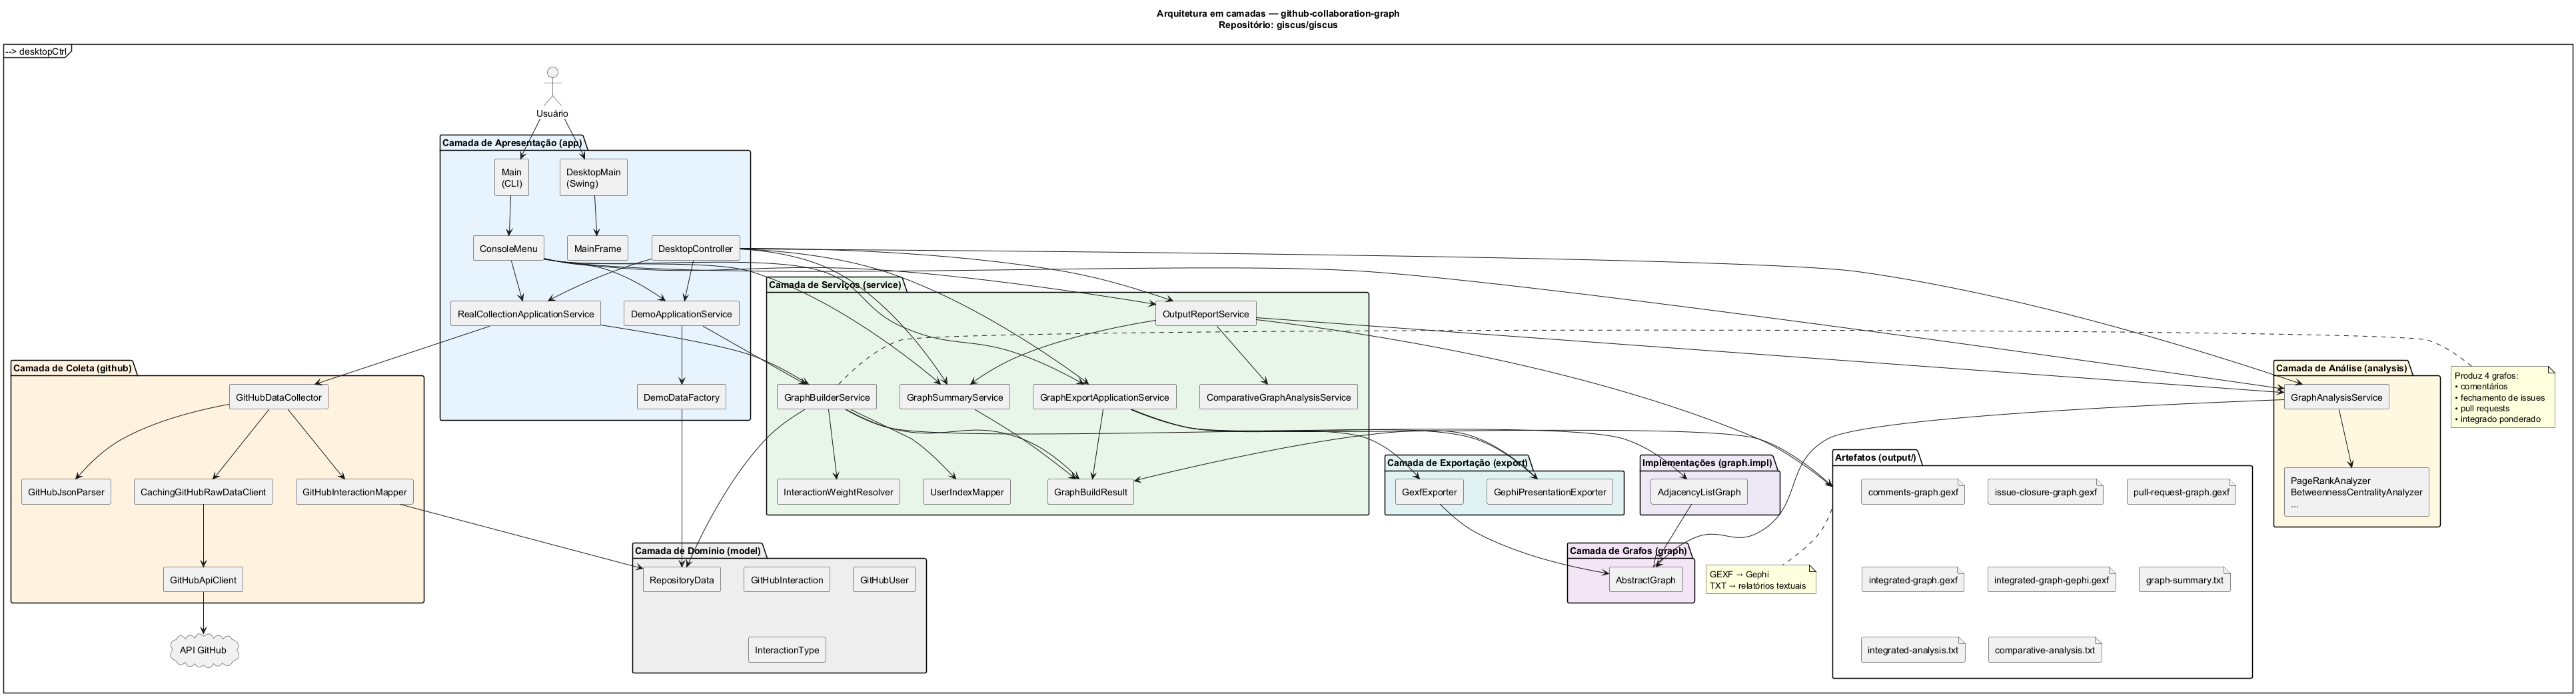
\includegraphics[width=0.8\textwidth]{Arquitetura_Camadas.png}
\caption{Arquitetura em Camadas e Fluxo de Dados do Sistema.} 
\label{fig:arquitetura}

  \vspace{0.2cm}
    \href{https://www.plantuml.com/plantuml/png/ZLVDRXit4BxlKn3EHJd8ITkaJNC8eiZQr4M26dQ21gXxe7P74cqkkU6FRQKja5CVeEWBf3tar5FH9z2R-4dA7wuqebPfVJ7dcsyuCvnPSlHK6wgCRNXXcE50HkgjPGQCLPH0GohQq9fgSll-Tp9dPc6dmqfoJgTIKSEa6CuLRHVduXHQgPbP_QsOVEoOkhBwNlnN5FgIYPOgsX2zeBMyPc9EPfHhG9fADgqK8CoPMRem55I6YZc7eg2LaOeSlDPszS7jVa1SE5PRwjP5qTBgaiw178n3eAHs6RGAjDk8hZwk_fHaGDlsRZ1o2t9dygXyK1wHdmgoSKb-U4cPE1U3yOlZkpzwQkFaRSPO2Yqvl0HX0wEAyZRf2FIbaMtQxSmd6lUhDufTnwNB7vBRAFLlwq8mId8E2kyvDehdz4QEsfQpAfJe3DGLgo3QHDKs_nGe7_jzAq_VOwaSARECdeweeMMeqNBj8id5Bxq5Shx0K3A8_HHh4zVaJbcMNqpkv-LvpimtTkezfJYbIaL8KXzzrB8nPmu8LDf9VTHljHGdLEbqiXThiOzyB0me6ixg9MtRPDE4PTOpj5gu5eXcf_JQ9u12gfmQehpdf8vai_fBC4a6ZQo1nwCAIzV8uIy_gVWT-iFtpcBb7EI5_yWbSDb6xgE_xax8xfmDskdLieMucr_jIItqrkgZr6IWOvl5x98GFjI7awztEi5VDyyiupKet9xJ26sJVRZ7eeORL2VMoPz8u7jWyuKv1ItvLJAx3f3U5upZMcusaKIvXtrccuQg9GvTHwY7FBbffJ9xFaZebDk6trdJMXUxLsAwYiXLbRMeMr9_bLz1S3aIb2yrqzYq2XpmjlsrT9OpNyZm5iGoXYMvupxcX-N3l8YZgJR-g8F7-7LYPClBSTDoQD9r_WzqNWwPmv4hJtCzSpJvglnonrrzGIiGrV85qzXdVU61FJcDnEe3Pnh8WAOZYTuwALnLZoQVvSxwJn4PxfJWn7a-fU8o6Bq3TIwUWRa640Aq7ZkAefoPvKPzU7WOTqo8tfD2R9_k6OGWnIJYsftN_VBpSZS5k9b5szJySmVab7R1Jj8xwpipuoUj3smc_OT93aPEFQF6zuaCFNelnXA54CECSPU0S-FhhOUnqDxvmLh9jBOmhBZKLa4lexMS3nMyjQ1D_nR2WCCDrFzBFGpPPAIeIL_keRanlVPToRS9rUQJonZkj5ncjdQ7TN9CufMBNaVte1L5cdp8SFWaJYaOm6E6LmQmcrIGqkDes5Yl0exdYY8QHqKQ0J0M1ueCIyU2CNHROHHz4nX7brM1ei51O1m7Wd4SJ8wZW78D3YhNuS2Ymm3ZcGVZtQiKWuvODxCW536BjJh0U4H0Qwz34qrS9HmrozPUQAh956bqYVyyiXaP2fJPjYO5l1_43ot6kvSKOzrLZ37yZYQzmtz-ahqLHIhmZiswm9_MnCijXxhxQrrlt4iPYlebqw27iq0ihqENTwR9ylFXzS8fn9tiibpYzOe2Gs0Xf06YV3s8dA4PwaJ9shuZ3yWylEoF7NJx_W-V3mWJVeNf1CsWMb2FIl_YXDkvK_cBcAIBkCFIvLXBqafHWryL86hY0qdXJAKnil7nf2W9UJvvKvBRNtyZuTbnmAithuAiWDFucrCJ0pV6KgOt-prrAzlmVm40}{Link PNG Arquitetura em Camadas}
\end{figure}

\subsection{Modelagem de Domínio}

O pacote \texttt{model} representa o problema independentemente da API de grafos da disciplina (Figura~\ref{fig:dominio}):

\begin{itemize}
\item \texttt{GitHubUser}: colaborador identificado pelo \textit{login};
\item \texttt{GitHubInteraction}: relação direcionada \texttt{sourceUser} $\rightarrow$ \texttt{targetUser} com \texttt{InteractionType};
\item \texttt{RepositoryData}: agregado com \textit{owner}, \textit{repository}, lista de interações e mapa de PRs abertos por autor;
\item \texttt{InteractionWeights}: constantes de peso (2, 3, 4, 5) alinhadas ao enunciado.
\end{itemize}

\begin{figure}[H]
\centering
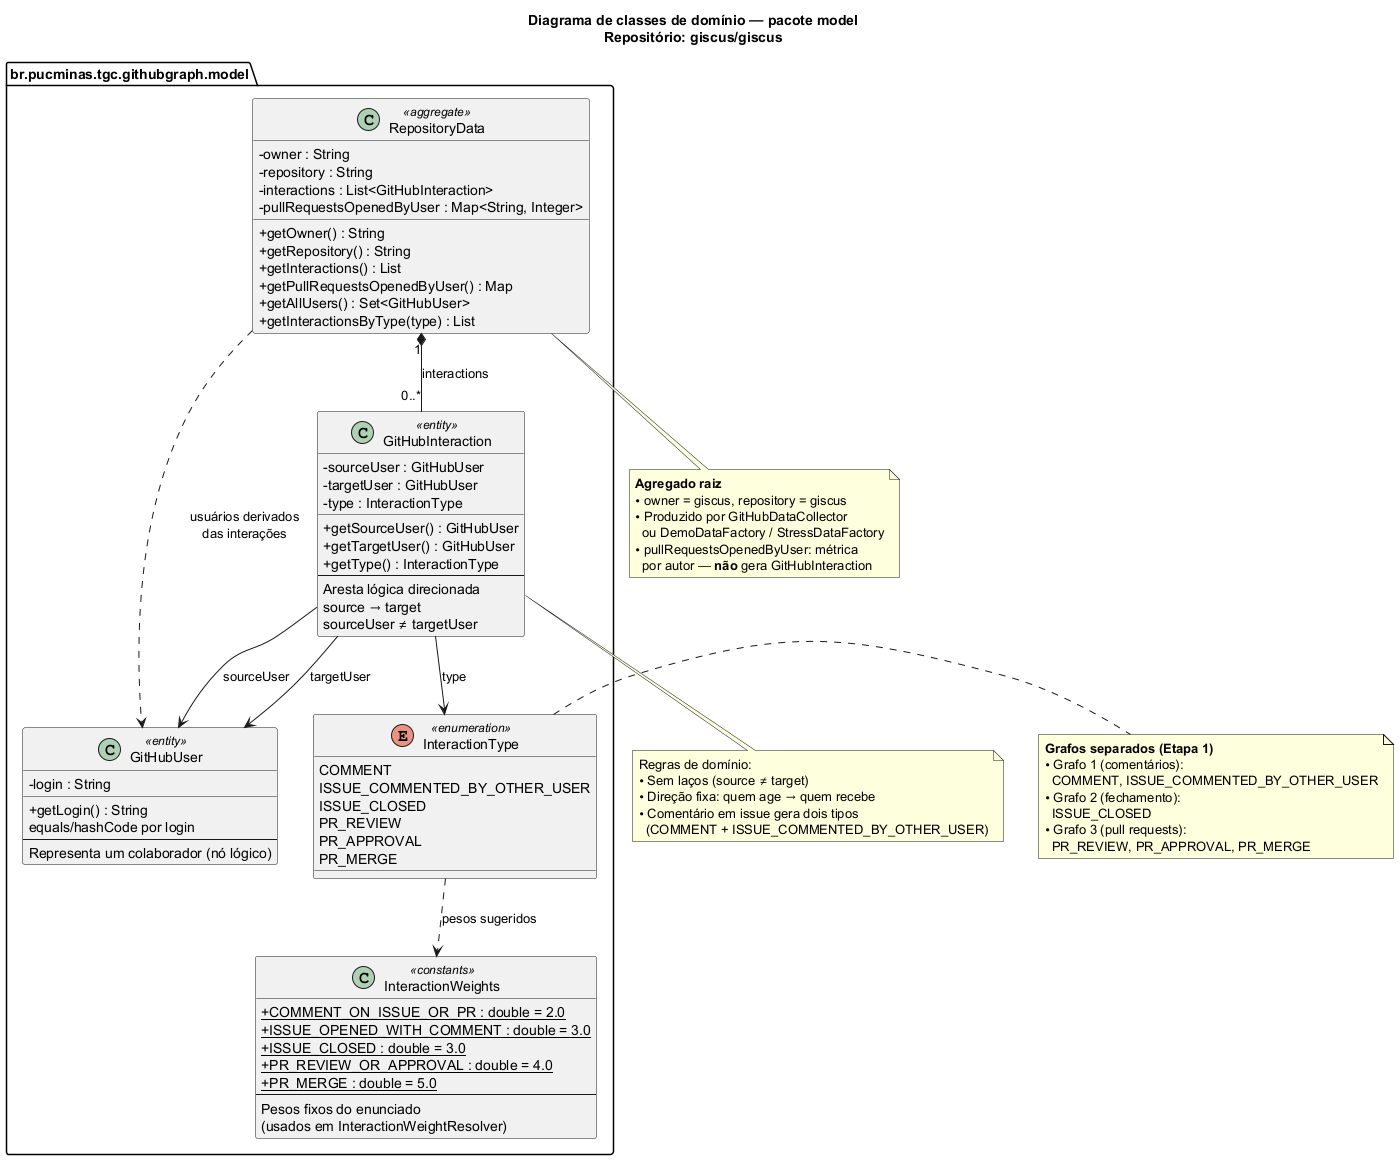
\includegraphics[width=0.6\textwidth]{Classes_Dominio.png}
\caption{Diagrama de Classes do Domínio.}
\label{fig:dominio}

  \vspace{0.2cm}
    \href{https://www.plantuml.com/plantuml/png/ZLRDRjj64BxhAGOwIOgjn4bx8HmXiiNQ1cnBeEmO1G8GAt9CBK9osTrbKZi8q5E1Nei-GDiSYXvwCle4UXC_IMUNjBGcbQGdaZlV_CmtEpDyfJIJkipIZkOwHPXmbaYMCOWHefGfXSgynY9R_PDp0VS__GO5YuH6o4ICwPiym48ehbTtaWiF4gwYKZsj7fsEUilpWf71ojXOQyaNfSQJIEHpVelmp86e9Ol5UvudSCrIXPqEENhB4eJkGWwBCifupjHG9z4muNfPBYZGOZcqONI1gIeW-D3fGEKDZhW-BXUN2YNixsDE6TwCHWG00DY5L2Gy1m_cMf9FUnY6zl444jIdHjphFmRW3oM5zdJ9rFAGl44XP6Mdihbh7yI8H4N-69IKk4ZPGaWM4xINh-uWNTqbF19zmduqiM9Eg9DSesIHvYA_k2dGn4l7T6HEra4VJi_E_FCB-tuodr_wONtYJyA3xyFfnR4VX9TpFt0HfzEvFx47io0C_DSd_jN3rtWs2wQlnwSFtsT-SEIRk9eSEk5jerA9KaPeYVOSrckfPfBu_ApKfEir2MYLOxvsqUktpLZ8XVNpPGYP9c7BdLk-iKIbMLqc1Z6N616CnSoAgrpX_kTVwyJCgSl0_I-_Eoa_PhDk5Y5l9ampef8bYSI4QNJO5EzpbEwzCuTohTcKy4qgYcIdNEdzLjL6DRWeqpIWMunAgsc1ESO7DtLbpbYnNndUiVGaA4UjCanDRCski99DQbl5JYoA05MS6_5iUrpagefiWnodgH6eoWi-v6hEHjlT7TpOifkBvZXsgkA0hv0dIwseCX5fQfPhjQxC1_hMFFf87kgs2wVdOTLbqo2S1MGy5kKYHNW9puVFcaerSkQVKxjUdLmSFtIlg_UYhUVsyLUWwmuFfvlkTdM-QUci-zw5VKimfoLcg8I2Q_wZK8Gn4okFE8k55VPAnM8IODOcCY35z1tAQjWHvQsBIIv6xg3sd5RwFsYdqxQZ6vrkL4p3TngjsDthmc1t5xhFXiD15zgsl4UDrbGV3XjnbQfS_I6v8GmbVsSOUfF7JDLMLd-j_aLQaCteoCwsw-X1OKkWoeIinO8qSxE35q9haO6uRamMedim6DlHGlMIZDyE1XsWxVrdFLrUrfjwnnaiwyCQEPCYBc_9crrpLNR6-A58Kun8mvPVb331J1Z1ToooTfwQxaUbdBFAv6V7ZmVPwcyjULJDMEEFbQHd_pS6WtprIGm6GBcpTcKwcCTWsAWvaOOoegHPUSl9aMJNXaSicBItjkThLZ3Owwy9iX3OWruaCinrLSM-voxWdQzjNyVGS-XTOxHanfOWCwtDx89VGCzG1BBcoE3TnRtZRksTTUisA72kHPijW00JoHxzrdbr47FC8AMxQNYfsj3PPlqQDE4IwVf-4cOWC0yeqWnOObTYzI4nmWNMyCCDYq0ohbI9LILZmHLeNWXLpP6QJNZoPNRxcsnVqLkPfVy1}{Link PNG Diagrama de Classes do Domínio}
\end{figure}

\subsection{Estratégia de Coleta e Mapeamento para Arestas}

A coleta opera em modo \texttt{FULL\_REPOSITORY}: paginação completa de issues, pull requests, comentários e revisões, com \textit{concurrency} configurável. A coleta possui suporte a cache local em \texttt{cache/github/}. Na execução de referência, os dados foram obtidos por mineração completa do repositório, sem reutilização prévia de respostas armazenadas em cache. Nessa execução foram processados 377 issues, 1054 pull requests, 4294 interações e 566 colaboradores distintos, em tempo de parede de aproximadamente 2min51s.

\begin{table}[H]
\centering
\caption{Transformação de eventos GitHub em interações e grafos.}
\small
\begin{tabular}{|p{3.5cm}|p{2.8cm}|p{2.1cm}|p{4.0cm}|}
\hline
\textbf{Evento GitHub} & \textbf{Origem $\rightarrow$ Destino} & \textbf{Grafo} & \textbf{Observação} \\
\hline Comentário em issue/PR & autor do comentário $\rightarrow$ autor do item & Comentários & Peso 2 no integrado \\
\hline Comentário de terceiro em issue & autor $\rightarrow$ autor da issue & Comentários & Gera também tipo com peso 3 \\
\hline Fechamento de issue & quem fechou $\rightarrow$ autor da issue & Fechamento & Peso 3 no integrado \\
\hline Review de PR & revisor $\rightarrow$ autor do PR & Pull requests & Peso 4 \\
\hline Aprovação de PR & revisor $\rightarrow$ autor do PR & Pull requests & Peso 4 \\
\hline Merge de PR & quem mergeou $\rightarrow$ autor do PR & Pull requests & Peso 5 \\
\hline Abertura de PR & -- & Nenhum & Contagem por autor (Tabela~\ref{tab:prs}) \\
\hline
\end{tabular}
\label{tab:mapeamento}
\end{table}

\subsection{Construção dos Quatro Grafos e Pesos}

O \texttt{GraphBuilderService} mapeia logins para índices inteiros via \texttt{UserIndexMapper} (ordem alfabética) e instancia quatro \texttt{AdjacencyListGraph}. Nos grafos \textbf{separados}, há no máximo uma aresta por par ordenado $(u,v)$, com peso fixo do tipo na primeira ocorrência. No grafo \textbf{integrado}, os pesos são \textbf{acumulados} quando o par já existe. O grafo é direcionado e simples: sem laços, sem arestas duplicadas no mesmo sentido; arestas antiparalelas $(u \rightarrow v)$ e $(v \rightarrow u)$ são permitidas.

\begin{table}[H]
\centering
\caption{Pesos fixos atribuídos por tipo de interação no grafo integrado.}
\vspace{0.2cm}
\begin{tabular}{|l|c|}
\hline
\textbf{Tipo de Interação} & \textbf{Peso} \\ \hline
Comentário em issue ou pull request & 2 \\ \hline
Comentário de terceiro em issue & 3 \\ \hline
Fechamento de issue & 3 \\ \hline
Revisão ou aprovação de pull request & 4 \\ \hline
Merge de pull request & 5 \\ \hline
\end{tabular}
\label{tab:pesos}
\end{table}

\begin{table}[H]
\centering
\caption{Contagem de vértices/arestas (mineração de referência).}
\vspace{0.2cm}
\begin{tabular}{|l|c|c|}
\hline
\textbf{Grafo} & \textbf{V} & \textbf{E} \\
\hline Comentários & 566 & 698 \\
\hline Fechamento de issues & 566 & 155 \\
\hline Pull requests & 566 & 51 \\
\hline Integrado ponderado & 566 & 737 \\
\hline
\end{tabular}
\label{tab:contagem_grafos}
\end{table}

\subsection{API Própria de Grafos}

Conforme exigido na Etapa~2, a estrutura topológica parte de \texttt{AbstractGraph}, com implementações \texttt{AdjacencyMatrixGraph} e \texttt{AdjacencyListGraph}. A API inclui contagem de vértices e arestas, consulta e mutação de arestas, relações estruturais (\texttt{isSucessor}, \texttt{isPredessor}, \texttt{isDivergent}, \texttt{isConvergent}, \texttt{isIncident}), graus, pesos de vértices e arestas, \texttt{isConnected}, \texttt{isEmptyGraph}, \texttt{isCompleteGraph} e \texttt{exportToGEPHI}. A operação \texttt{addEdge} é idempotente; índices inválidos e laços lançam exceções.

\begin{figure}[H]
\centering
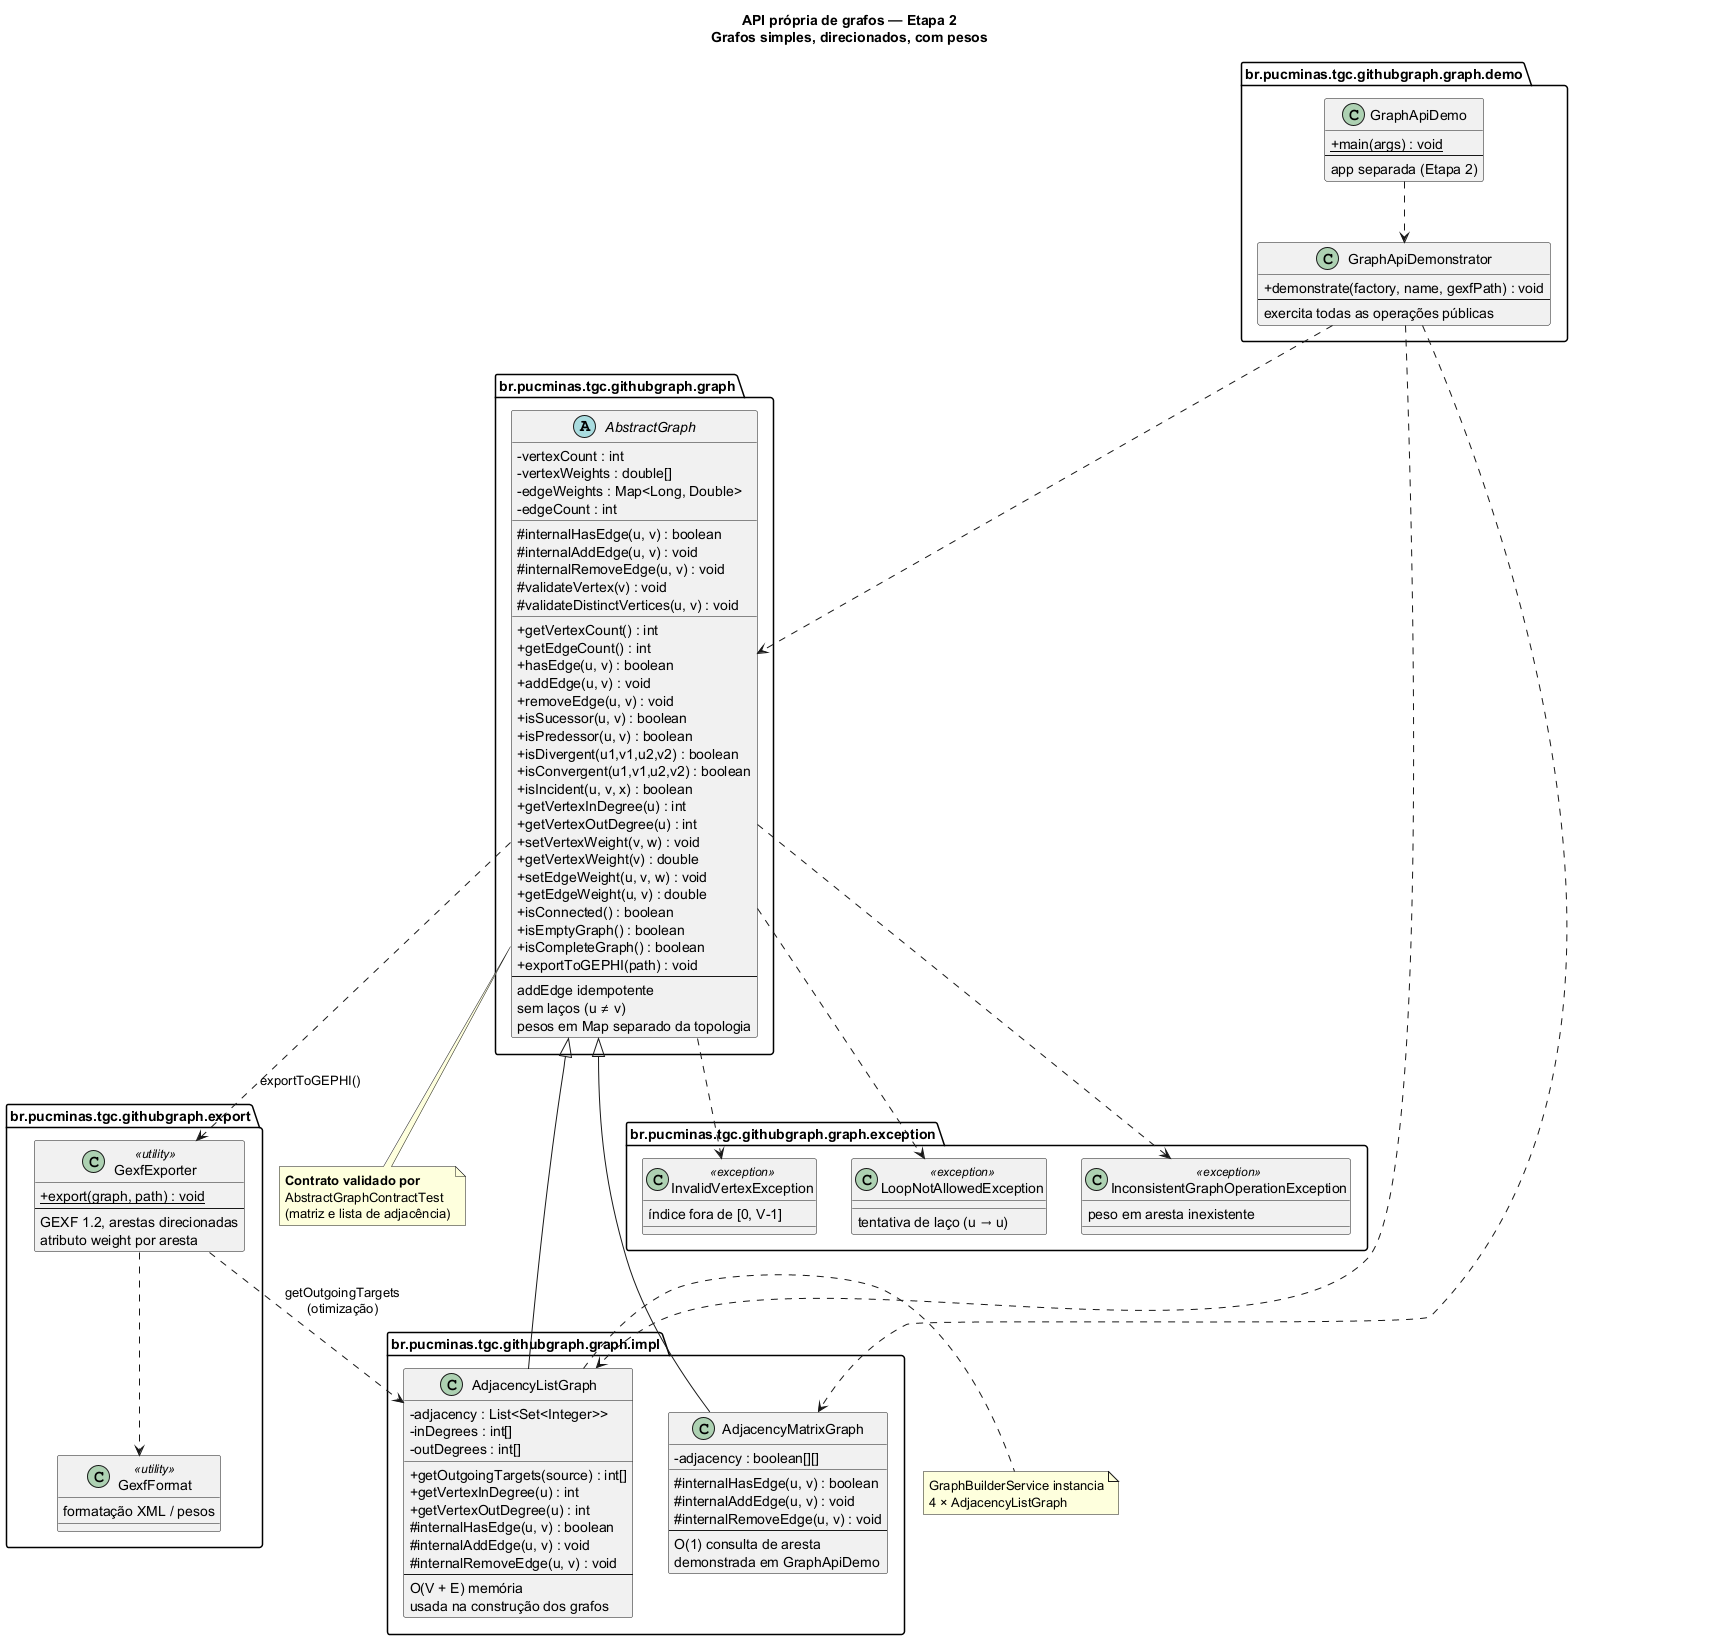
\includegraphics[width=0.8\textwidth]{Classes_API.png}
\caption{Diagrama de Classes da API de Grafos}
\label{fig:diagrama_classes}

\vspace{0.2cm}
    \href{https://www.plantuml.com/plantuml/png/nLP1RnH74xtFhoZnNMRDUZzivOIi5GvUp4ecM34YI81GxNJjR8UPxb5tpNeDGSefKgvHf5mZvO0KAIUKIwxxJ_WbcUvf3vwb5m4vSB5dkjvMrNjT_NfkMKR3TLaaBBaWE3oTGcNMRoeZ4GH1Rd2kBRpzyLUOC5O8-q_KSRjcPLaLP8SWfA5CQeL2Ds-PBg4YgssIsETILMYmXAn0Qm-PZPpLJDDCgpFvWk365OXTeD3dKkKmny9IabIOFSUSuDhCZAewAwL2E-8y6-MI5_MiwQnQZFpVQu0M_1EyJ180d5asc75R5Wx3wt50003imf8Cq-gshXN3JP2AU-lVaSmNR9k8qFMieCTFGvX4Jk-2zx0wED4g7yAHXusle3PJFtlc__tFBP1HMDn5EsbmQJs4vQ01phGk2DK6wb287cgffTY0V4kbNj8sr18BAP3feIUMRWiVISjIPUnWCYExcQeZS1roygYWNZe89BkWwoGMMiG9XoX6YVgGYHCCKMdFweoirMPBPcbF3OaF8uxaaanEJS_rtd2vDwptXylz6F2sLX-9dAfCYWRdQmvXrSFqXPog8yeDDVJwYdM0-pN74JOWmiIcJQ7p3NtoJSYW6-jtIIRTNFjserdwc7wQJXn56PD8Ou9Coeel_2bCuyewGs7QXg1LfGq_qCUJqxlJj49Uz5hStVN_mXY155HMcabnsvwb4WfSlzOMqXhU_lnxGy07l5a1bUumDoZdHaA3G61TwKBd4XlOg-JLfpZIo7cZjoNtqBfIC2FnFMQaieiJQJSS2Iz33IiNFJWZFfWgffpCU1n0CaoARQUWyoLTSoJGExFD3ELQglm1ckRDfbRN9gD1X__lC_ab32vi-_tqOTFRP00bbUitHg9VhIqA18MGQMNPrElNwpyq26t3nUPsDh8tzv2DN6tVdK3ayTDEvI_AV6_W-TK5-piR3Lbk-GigFN6d0fNW6HrMygXP_eoXfbL65Kkj_6GtRrS7UwhyJTAEnkGI2GS7tQ_6uo3c-YybP4OmryOt_FZ641xkxZtjxyQ9rjKtcW-BGf-J-7169iN8SkdJ-LFk3_bFlq0zw6UTAYULjEuNNexx5HbqoRPMw5m2g0pYWbIqQfFG9mdPUbZGpprUbV2OLlE9NoNJD56pB2HVT2syj8vZzggpmjJd7C8sApoUFBe3UwFzOUZQNlbKG-iXs7wIQJZtlWvDsW3sj7gjtT6cH8uqDlS1R0_NetidyF_ML3zZnDp0UdNSGq-RRdJ3HBCseVnr4DqYfNFCcj3541IMD8IyQVnqYpwq8fD9Hc0jqBggkYBZUFnD5ghrFxD2PkXfn1jvVsDAb2f5azjOFQow2mOX3T_JWqkL8ZV3Rbtj_Z3kVy0cKPUA8fFUAun6u_w8tTouKWT9BnpmOT_VZqKQlXcvPvweLBCivOjsG0QnjkBc4G76JI62_9Y3dYIzpVHy8sEMn1OzkbSr3eiBjHqRszqaKPe9PffPbw3d6tK1TdPkQ-MJXCzveTr9tjb9e8zjOHa_8CjDB2rTaHT0K4WRBWzNV_sdoYGE4b82NEdGWF4MeUSnGj1AztKj2q7cZCpIERnKbj7bQk9VmVgts2-x8hUQfxei_WK0}{Link PNG Diagrama de Classes da API}
\end{figure}

\texttt{AdjacencyMatrixGraph} favorece verificação $O(1)$ de arestas; \texttt{AdjacencyListGraph} otimiza memória em $O(V+E)$ e é a representação usada na construção dos grafos de colaboração.

\subsection{Interfaces e Demonstração}

Três pontos de entrada consomem a mesma camada de serviços:

\begin{enumerate}
\item \textbf{CLI (\texttt{Main}):} menu interativo para mineração real, demonstração offline (contingência), resumo dos grafos, análise de métricas e exportação GEXF;
\item \textbf{Desktop Swing (\texttt{DesktopMain}):} interface gráfica com \textit{SwingWorkers}, barra de progresso e logs da mineração em segundo plano;
\item \textbf{\texttt{GraphApiDemo}:} aplicação \textbf{separada} que instancia matriz e lista de adjacência e demonstra \textbf{todas} as operações públicas de \texttt{AbstractGraph}, incluindo validações e \texttt{exportToGEPHI}.
\end{enumerate}

\begin{figure}[H]
    \centering
    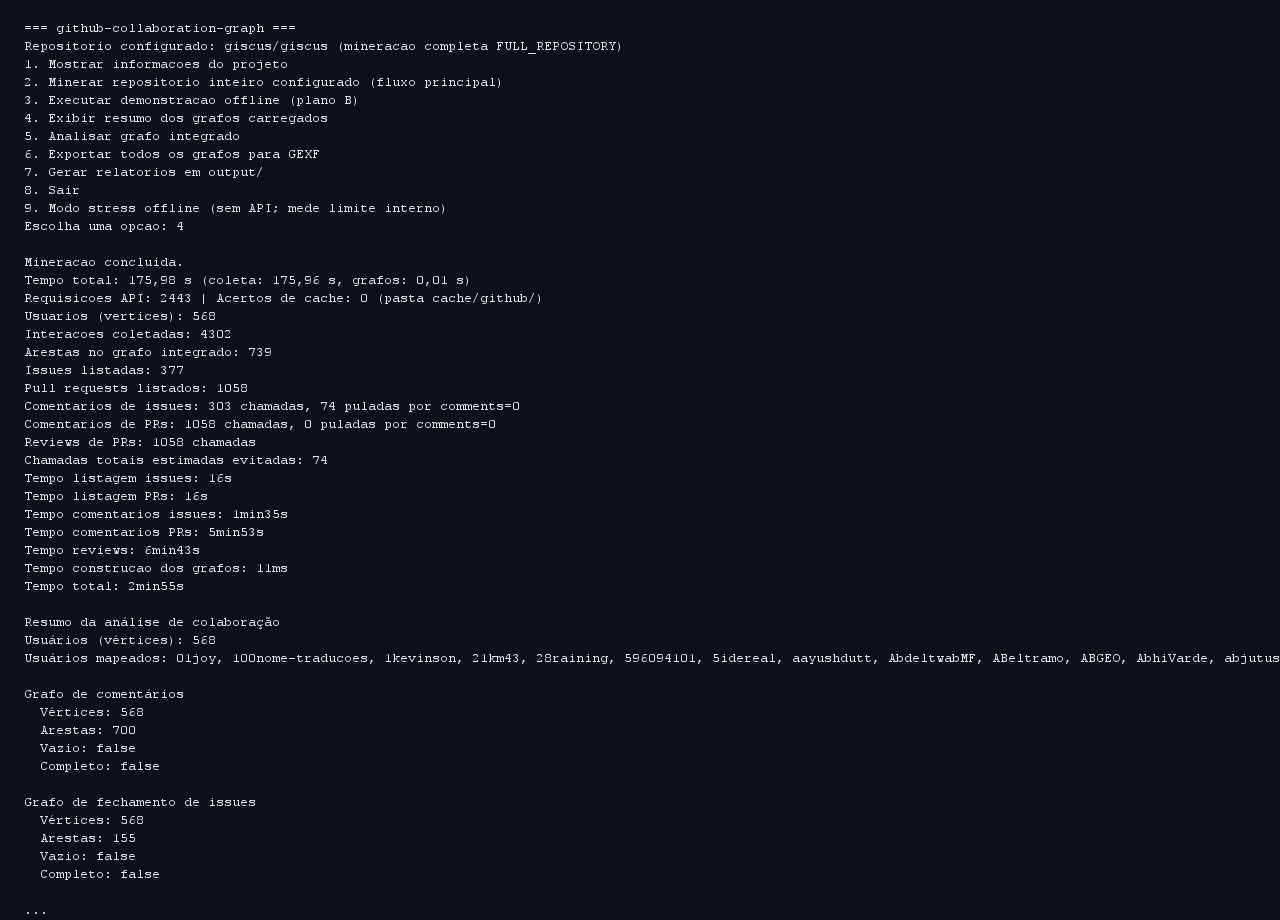
\includegraphics[width=0.8\textwidth]{tela_cli.png}
    \caption{Interface CLI (Menu interativo no terminal) para execução da mineração.}
    \label{fig:tela_cli}
\end{figure}
\begin{figure}[H]
    \centering
    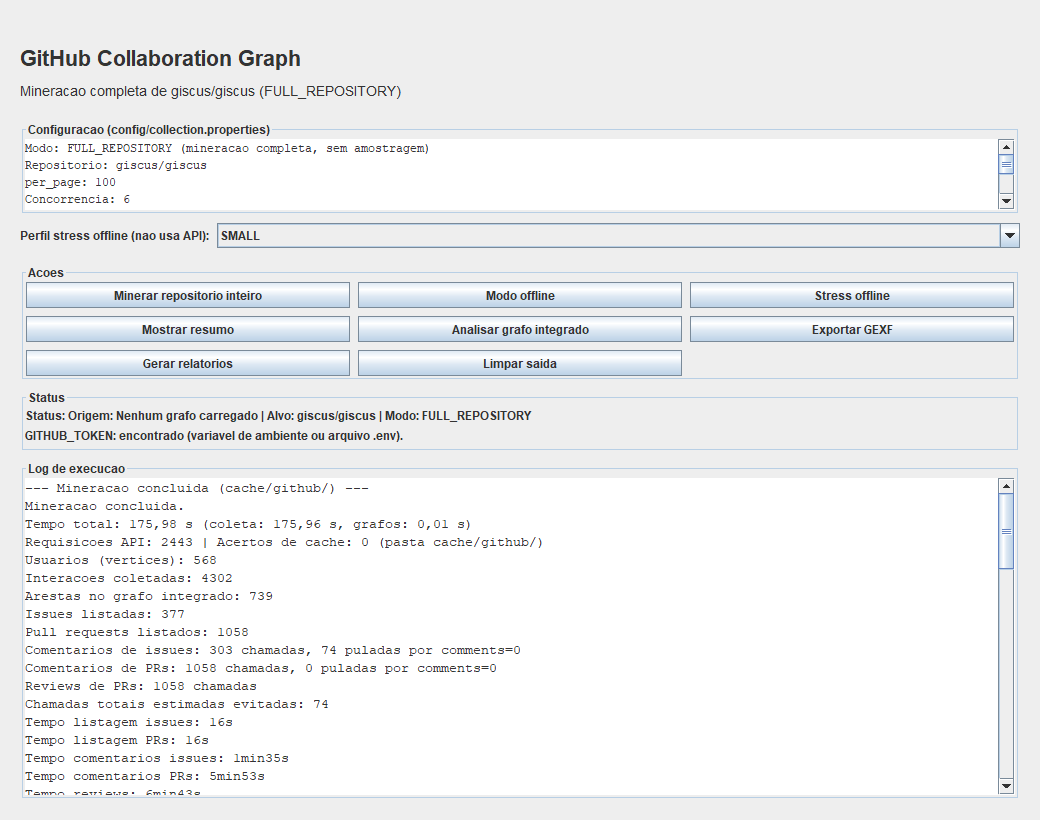
\includegraphics[width=0.8\textwidth]{tela_desktop.png}
    \caption{Interface Gráfica Desktop desenvolvida em Java Swing exibindo logs de extração.}
    \label{fig:tela_desktop}
\end{figure}

\subsection{Validação e Testes}

O projeto possui \textbf{167 testes unitários} (JUnit~5), executados offline. Destacam-se: \texttt{AbstractGraphContractTest} (contrato da API para matriz e lista); \texttt{GitHubInteractionMapperTest} e \texttt{GitHubDataCollectorTest} (mineração e mapeamento); \texttt{GraphBuilderServiceTest} (quatro grafos e pesos acumulados); testes dos analisadores (PageRank, Brandes, comunidades, \textit{bridging ties}); \texttt{GexfExporterTest} e \texttt{GraphApiDemonstratorTest}. Nenhum teste depende da API real do GitHub.

\section{Métricas e Algoritmos Implementados}
\label{sec:metricas}

Todas as métricas são calculadas manualmente sobre o grafo integrado, sem JGraphT, NetworkX ou equivalentes. O \texttt{GraphAnalysisService} orquestra onze blocos de análise, materializados no arquivo \texttt{integrated-analysis.txt}:

\begin{multicols}{2}
\begin{enumerate}[label=\arabic*., nosep]
  \item \textbf{Grau (Degree):} graus de entrada, saída e total;
  \item \textbf{Densidade:} $E / (V(V-1))$ para grafo direcionado simples;
  \item \textbf{PageRank:} iteração com \textit{damping} 0,85; em grafo direcionado, mede centralidade recebida na rede;
  \item \textbf{Centralidade de autovetor:} \textit{power iteration} nas arestas de entrada; indica relevância como destino das interações;
  \item \textbf{Closeness:} BFS direcional para caminhos mínimos não ponderados, com tratamento específico para vértices inalcançáveis em grafos desconexos;
  \item \textbf{Betweenness (Brandes):} caminhos mínimos em grafo direcionado não ponderado;
  \item \textbf{Clustering:} coeficiente local médio em vizinhança fraca;
  \item \textbf{Assortatividade:} correlação de Pearson entre graus totais fracos dos extremos das arestas;
  \item \textbf{Comunidades:} \textit{label propagation} determinístico + modularidade aproximada;
  \item \textbf{Bridging ties (laços-ponte):} arestas entre comunidades distintas ranqueadas por score;
  \item \textbf{Aberturas de PR:} contagem por autor (sem aresta no grafo).
\end{enumerate}
\end{multicols}

Em grafos com mais de 8.000 vértices, métricas pesadas (eigenvector, closeness, betweenness, comunidades) podem ser omitidas automaticamente; no \texttt{giscus/giscus} (566 vértices), todas foram calculadas.

\section{Resultados e Análise}
\label{sec:resultados}

A mineração integral produziu a rede da Tabela~\ref{tab:estrutura}. A densidade global foi de \textbf{0,0023}, indicando rede esparsa típica de OSS. O coeficiente médio de aglomeração foi \textbf{0,1949} e a assortatividade \textbf{$-0{,}2767$}, sugerindo que colaboradores de graus diferentes tendem a interagir entre si.

\subsection{Análise Visual dos Grafos}

As Figuras~\ref{fig:grafo_comentarios}--\ref{fig:grafo_integrado} foram geradas a partir dos arquivos GEXF exportados pela ferramenta; o grafo integrado reutiliza o layout do \texttt{integrated-graph-gephi.gexf} (Gephi), com \textit{logins} reais. O grafo de comentários é o mais denso (698 arestas); o de fechamento concentra mantenedores (155); o de PRs isola revisão e merge (51); o integrado consolida pesos acumulados (737).

\begin{figure}[H]
    \centering
    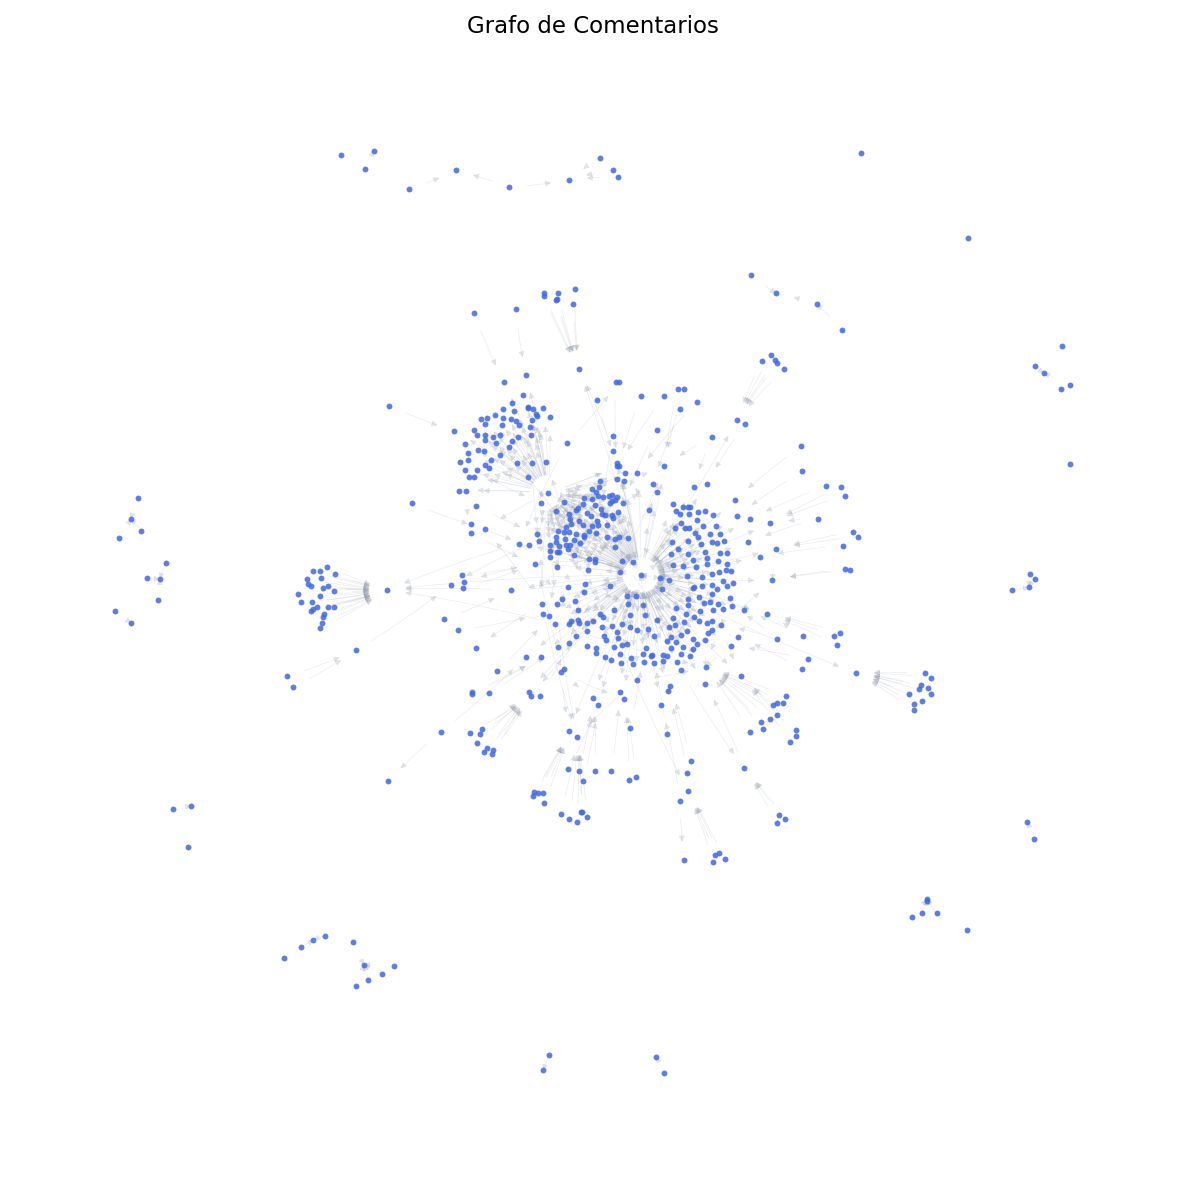
\includegraphics[width=0.4\textwidth]{grafo_comentarios.png}
    \caption{Visualização da sub-rede correspondente ao Grafo de Comentários.}
    \label{fig:grafo_comentarios}
\end{figure}

\begin{figure}[H]
    \centering
    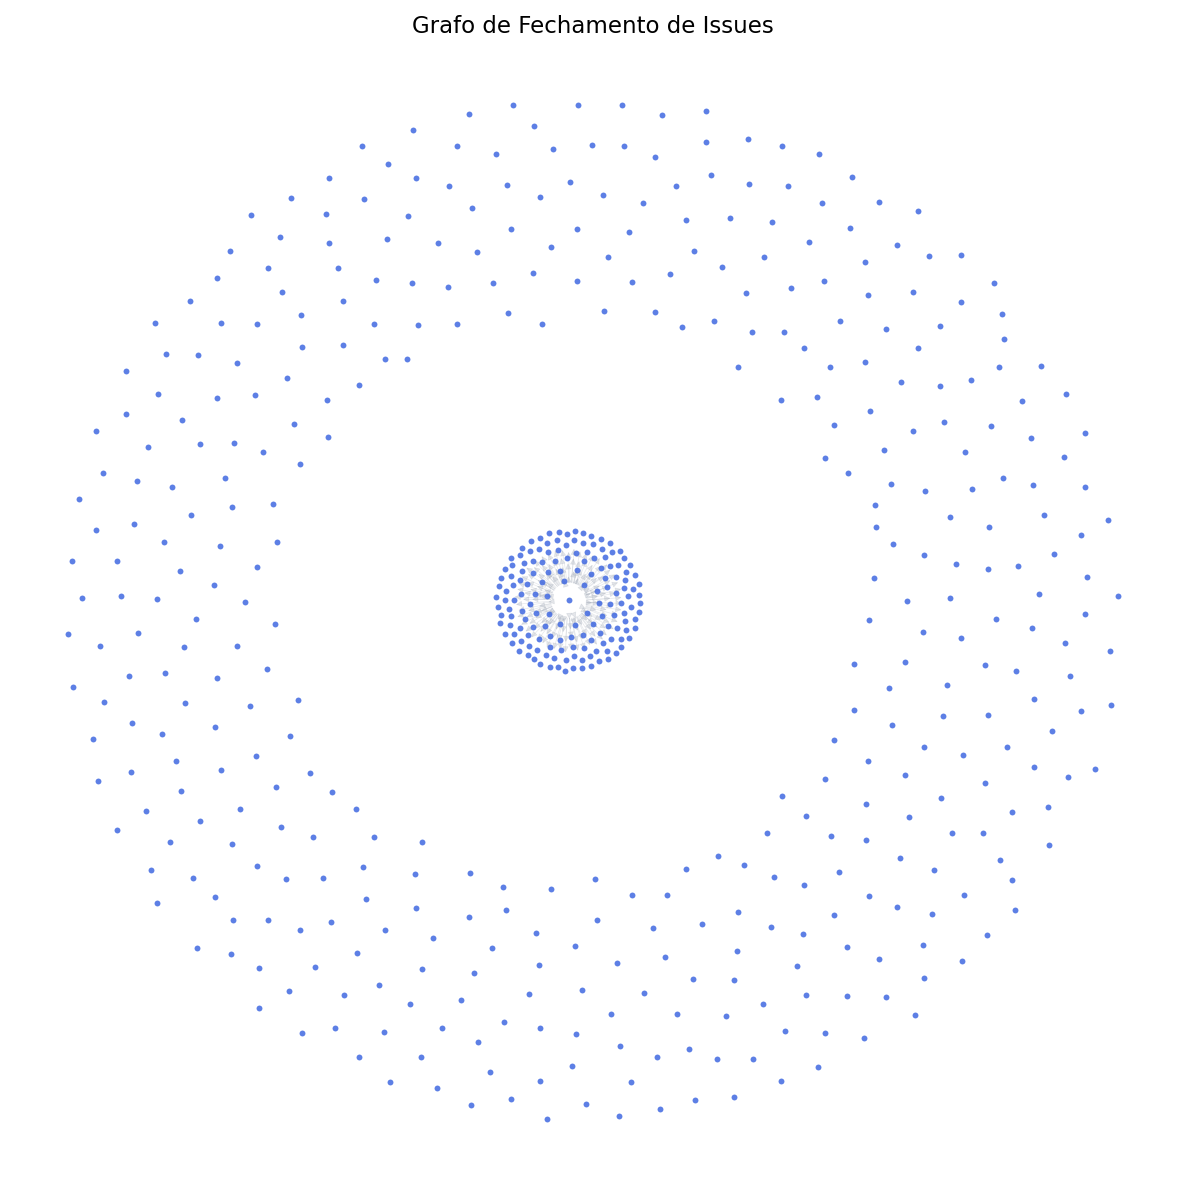
\includegraphics[width=0.4\textwidth]{grafo_fechamento.png}
    \caption{Visualização do Grafo de Fechamento de Issues.}
    \label{fig:grafo_fechamento}
\end{figure}

\begin{figure}[H]
    \centering
    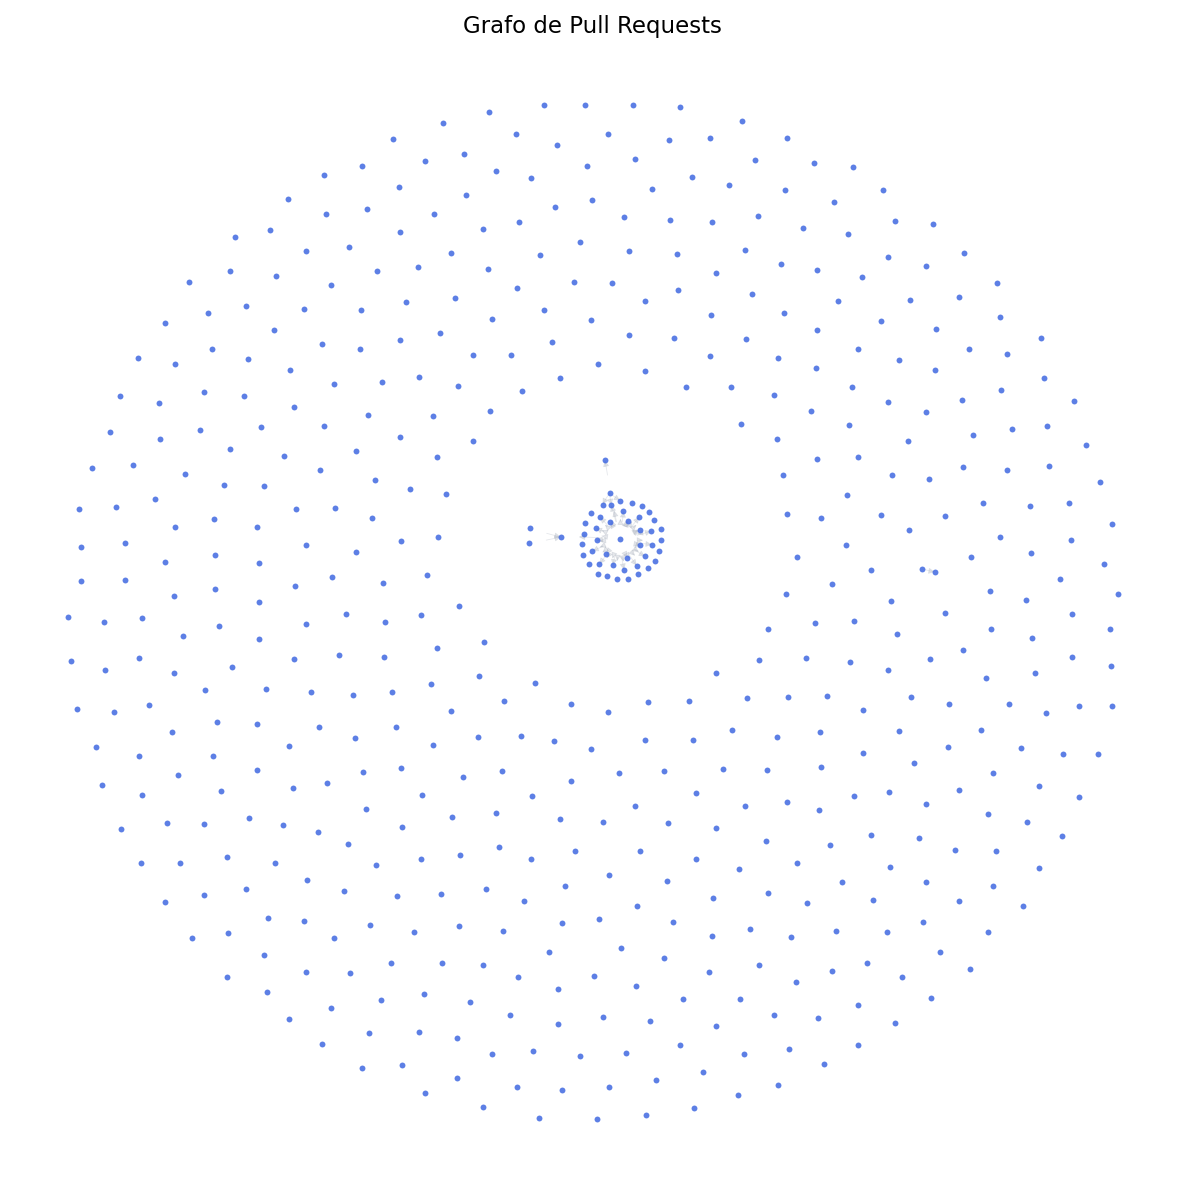
\includegraphics[width=0.4\textwidth]{grafo_pr.png}
    \caption{Visualização do Grafo focado em Revisões e Merges de Pull Requests.}
    \label{fig:grafo_pr}
\end{figure}

\begin{figure}[H]
    \centering
    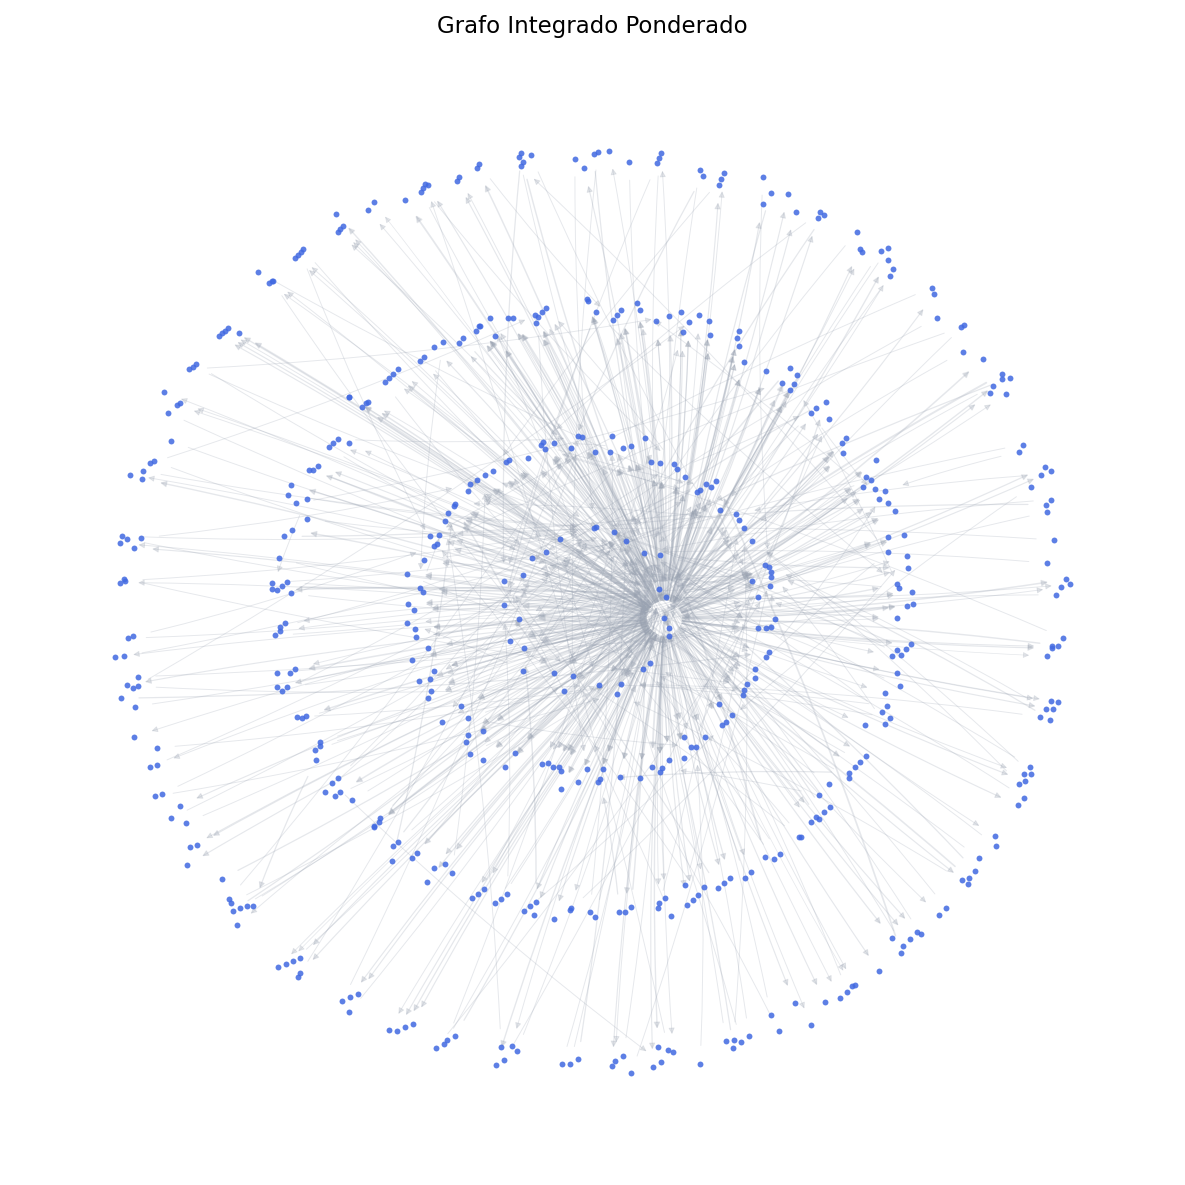
\includegraphics[width=0.4\textwidth]{grafo_integrado.png}
    \caption{Visualização do Grafo Integrado Ponderado completo.}
    \label{fig:grafo_integrado}
\end{figure}

\subsection{Métricas Globais e de Estrutura}
\label{sec:metricas_estrutura}

\begin{table}[H]
\centering
\caption{Métricas globais e estruturais do grafo integrado.}
\small
\begin{tabular}{|l|c|}
\hline
\textbf{Métrica} & \textbf{Valor} \\
\hline Vértices & 566 \\
\hline Arestas & 737 \\
\hline Densidade & 0,0023 \\
\hline Clustering (média) & 0,1949 \\
\hline Assortatividade (Pearson) & $-0{,}2767$ \\
\hline Comunidades detectadas & 37 \\
\hline Maior comunidade & 370 vértices (65,37\%) \\
\hline Modularidade (aprox.) & 0,3563 \\
\hline PRs abertos (total) & 1054 \\
\hline
\end{tabular}
\label{tab:estrutura}
\end{table}

A detecção de comunidades identificou um núcleo dominante (comunidade 265, centrada em \textit{laymonage}, com 370 membros incluindo \textit{vercel[bot]} e \textit{nschonni}) e comunidades menores (ex.: comunidade 90 com \textit{CheeseB}, 31 membros).

\subsection{Centralidades Estruturais}

A Tabela~\ref{tab:grau} apresenta os cinco primeiros colaboradores em métricas de centralidade. Como cada aresta segue a direção autor da ação $\rightarrow$ usuário associado ao artefato afetado, PageRank e centralidade de autovetor devem ser lidos como centralidade recebida ou relevância como destino das interações, e não como prova de influência direta. O usuário \textit{laymonage} lidera grau total (338), betweenness (15262,33) e PageRank (0,0428), indicando posição estrutural central na rede de interações observada. \textit{vercel[bot]} aparece em segundo no grau (131), reflexo de automação de \textit{deploy}.

\begin{table}[H]
\centering
\caption{Top 5 colaboradores por centralidade estrutural.}
\small
\begin{minipage}[t]{0.48\textwidth}
\centering
\textbf{Grau total}\\[2pt]
\begin{tabular}{|l|c|c|}
\hline
\textbf{Usuário} & \textbf{Grau} & \textbf{Rank} \\
\hline laymonage & 338 & 1 \\
\hline vercel[bot] & 131 & 2 \\
\hline CheeseB & 28 & 3 \\
\hline nschonni & 18 & 4 \\
\hline marcosruiz & 16 & 5 \\
\hline
\end{tabular}
\label{tab:grau}
\end{minipage}\hfill
\begin{minipage}[t]{0.48\textwidth}
\centering
\textbf{Betweenness (Brandes)}\\[2pt]
\begin{tabular}{|l|c|c|}
\hline
\textbf{Usuário} & \textbf{Score} & \textbf{Rank} \\
\hline laymonage & 15262,3333 & 1 \\
\hline ghost & 604,0000 & 2 \\
\hline williamhorning & 445,5000 & 3 \\
\hline ouuan & 303,5000 & 4 \\
\hline sohang3112 & 303,0000 & 5 \\
\hline
\end{tabular}
\label{tab:betweenness}
\end{minipage}

\vspace{6pt}

\begin{minipage}[t]{0.48\textwidth}
\centering
\textbf{PageRank}\\[2pt]
\begin{tabular}{|l|c|c|}
\hline
\textbf{Usuário} & \textbf{Score} & \textbf{Rank} \\
\hline laymonage & 0,0428 & 1 \\
\hline CheeseB & 0,0288 & 2 \\
\hline marcosruiz & 0,0157 & 3 \\
\hline antulik & 0,0114 & 4 \\
\hline ceynri & 0,0095 & 5 \\
\hline
\end{tabular}
\label{tab:pagerank}
\end{minipage}\hfill
\begin{minipage}[t]{0.48\textwidth}
\centering
\textbf{Eigenvector}\\[2pt]
\begin{tabular}{|l|c|c|}
\hline
\textbf{Usuário} & \textbf{Score} & \textbf{Rank} \\
\hline laymonage & 0,2099 & 1 \\
\hline marcosruiz & 0,1374 & 2 \\
\hline CheeseB & 0,1104 & 3 \\
\hline refparo & 0,0970 & 4 \\
\hline Canfry & 0,0835 & 5 \\
\hline
\end{tabular}
\label{tab:eigenvector}
\end{minipage}
\end{table}

\textbf{Closeness:} Closeness foi mantida por completude, mas em grafos direcionados esparsos seu ranking pode destacar vértices periféricos localizados em componentes pequenas. Por isso, seus resultados devem ser interpretados junto com grau, PageRank e betweenness, evitando conclusões isoladas sobre centralidade global.

\subsection{Bridging Ties e Aberturas de PR}

As bridging ties (laços-ponte) mais relevantes conectam a comunidade principal (265) a comunidades menores. Exemplos: \textit{laymonage} $\rightarrow$ \textit{CheeseB} (comunidades 265/90, peso 13,0); \textit{laymonage} $\rightarrow$ \textit{pourmand1376} (265/90, peso 16,0); \textit{ghost} $\rightarrow$ \textit{laymonage} (158/265, peso 10,0). Essas arestas indicam colaboradores que funcionam como pontes entre grupos que, de outra forma, interagiriam pouco.

\begin{table}[H]
\centering
\caption{Top 5 -- Aberturas de pull requests (métrica sem aresta).}
\small
\begin{tabular}{|l|c|}
\hline
\textbf{Usuário} & \textbf{PRs abertos} \\
\hline dependabot[bot] & 674 \\
\hline laymonage & 213 \\
\hline nschonni & 10 \\
\hline nidexingg & 5 \\
\hline Andre601 & 3 \\
\hline
\end{tabular}
\label{tab:prs}
\end{table}

A predominância de \textit{dependabot[bot]} reflete automação de dependências; \textit{laymonage} lidera entre contribuidores humanos na abertura de PRs.

\section{Conclusão}
A análise do repositório \texttt{giscus/giscus} demonstrou que a ferramenta desenvolvida compila dados heterogêneos de colaboração em redes direcionadas analisáveis. Os quatro grafos permitiram separar comunicação (698 arestas), fechamento e gerenciamento de issues (155), revisão técnica (51) e visão integrada ponderada (737).

Os resultados indicam comunicação amplamente distribuída em comentários, mas concentração de revisão, \textit{merge} e fechamento em poucos mantenedores, notadamente \textit{laymonage}, com posição estrutural destacada em grau, betweenness, PageRank e centralidade de autovetor. Métricas estruturais reforçam rede esparsa (densidade 0,0023), assortatividade negativa e comunidade principal com 65\,\% dos vértices.

A implementação nativa da API de grafos, validada por 167 testes e pela aplicação \texttt{GraphApiDemo}, atende aos requisitos das três etapas do trabalho. A exportação GEXF e as onze métricas topológicas transformam a ferramenta em instrumento de análise visual e quantitativa aplicável a outros ecossistemas open source de porte semelhante.

\bibliographystyle{sbc}
\bibliography{sbc-template}
\end{document}